\section{The First G-APD Cherenkov Telescope}

\begin{frame}{The FACT Experiment}
    \begin{columns}[T] % align columns
        \begin{column}{.45\textwidth}
            \vspace{10pt}
            \begin{itemize}
                \item ``First G-APD Cherenkov Telescope"
                \item Operating on La Palma since 2011
                \item Monoscopic reconstruction only
                \item Advanced analysis pipeline
                \item What did we take a look at?
                \begin{itemize}
                    \item{More advanced cleaning method}
                    \item{Distinction of "islands" in shower images}
                    \item[\rightarrow] Possible improvements for monoscopic reconstruction in ctapipe
                    \item[\rightarrow] First use case: LST1
                \end{itemize}
            \end{itemize}
        \end{column}
        \begin{column}{.48\textwidth}
            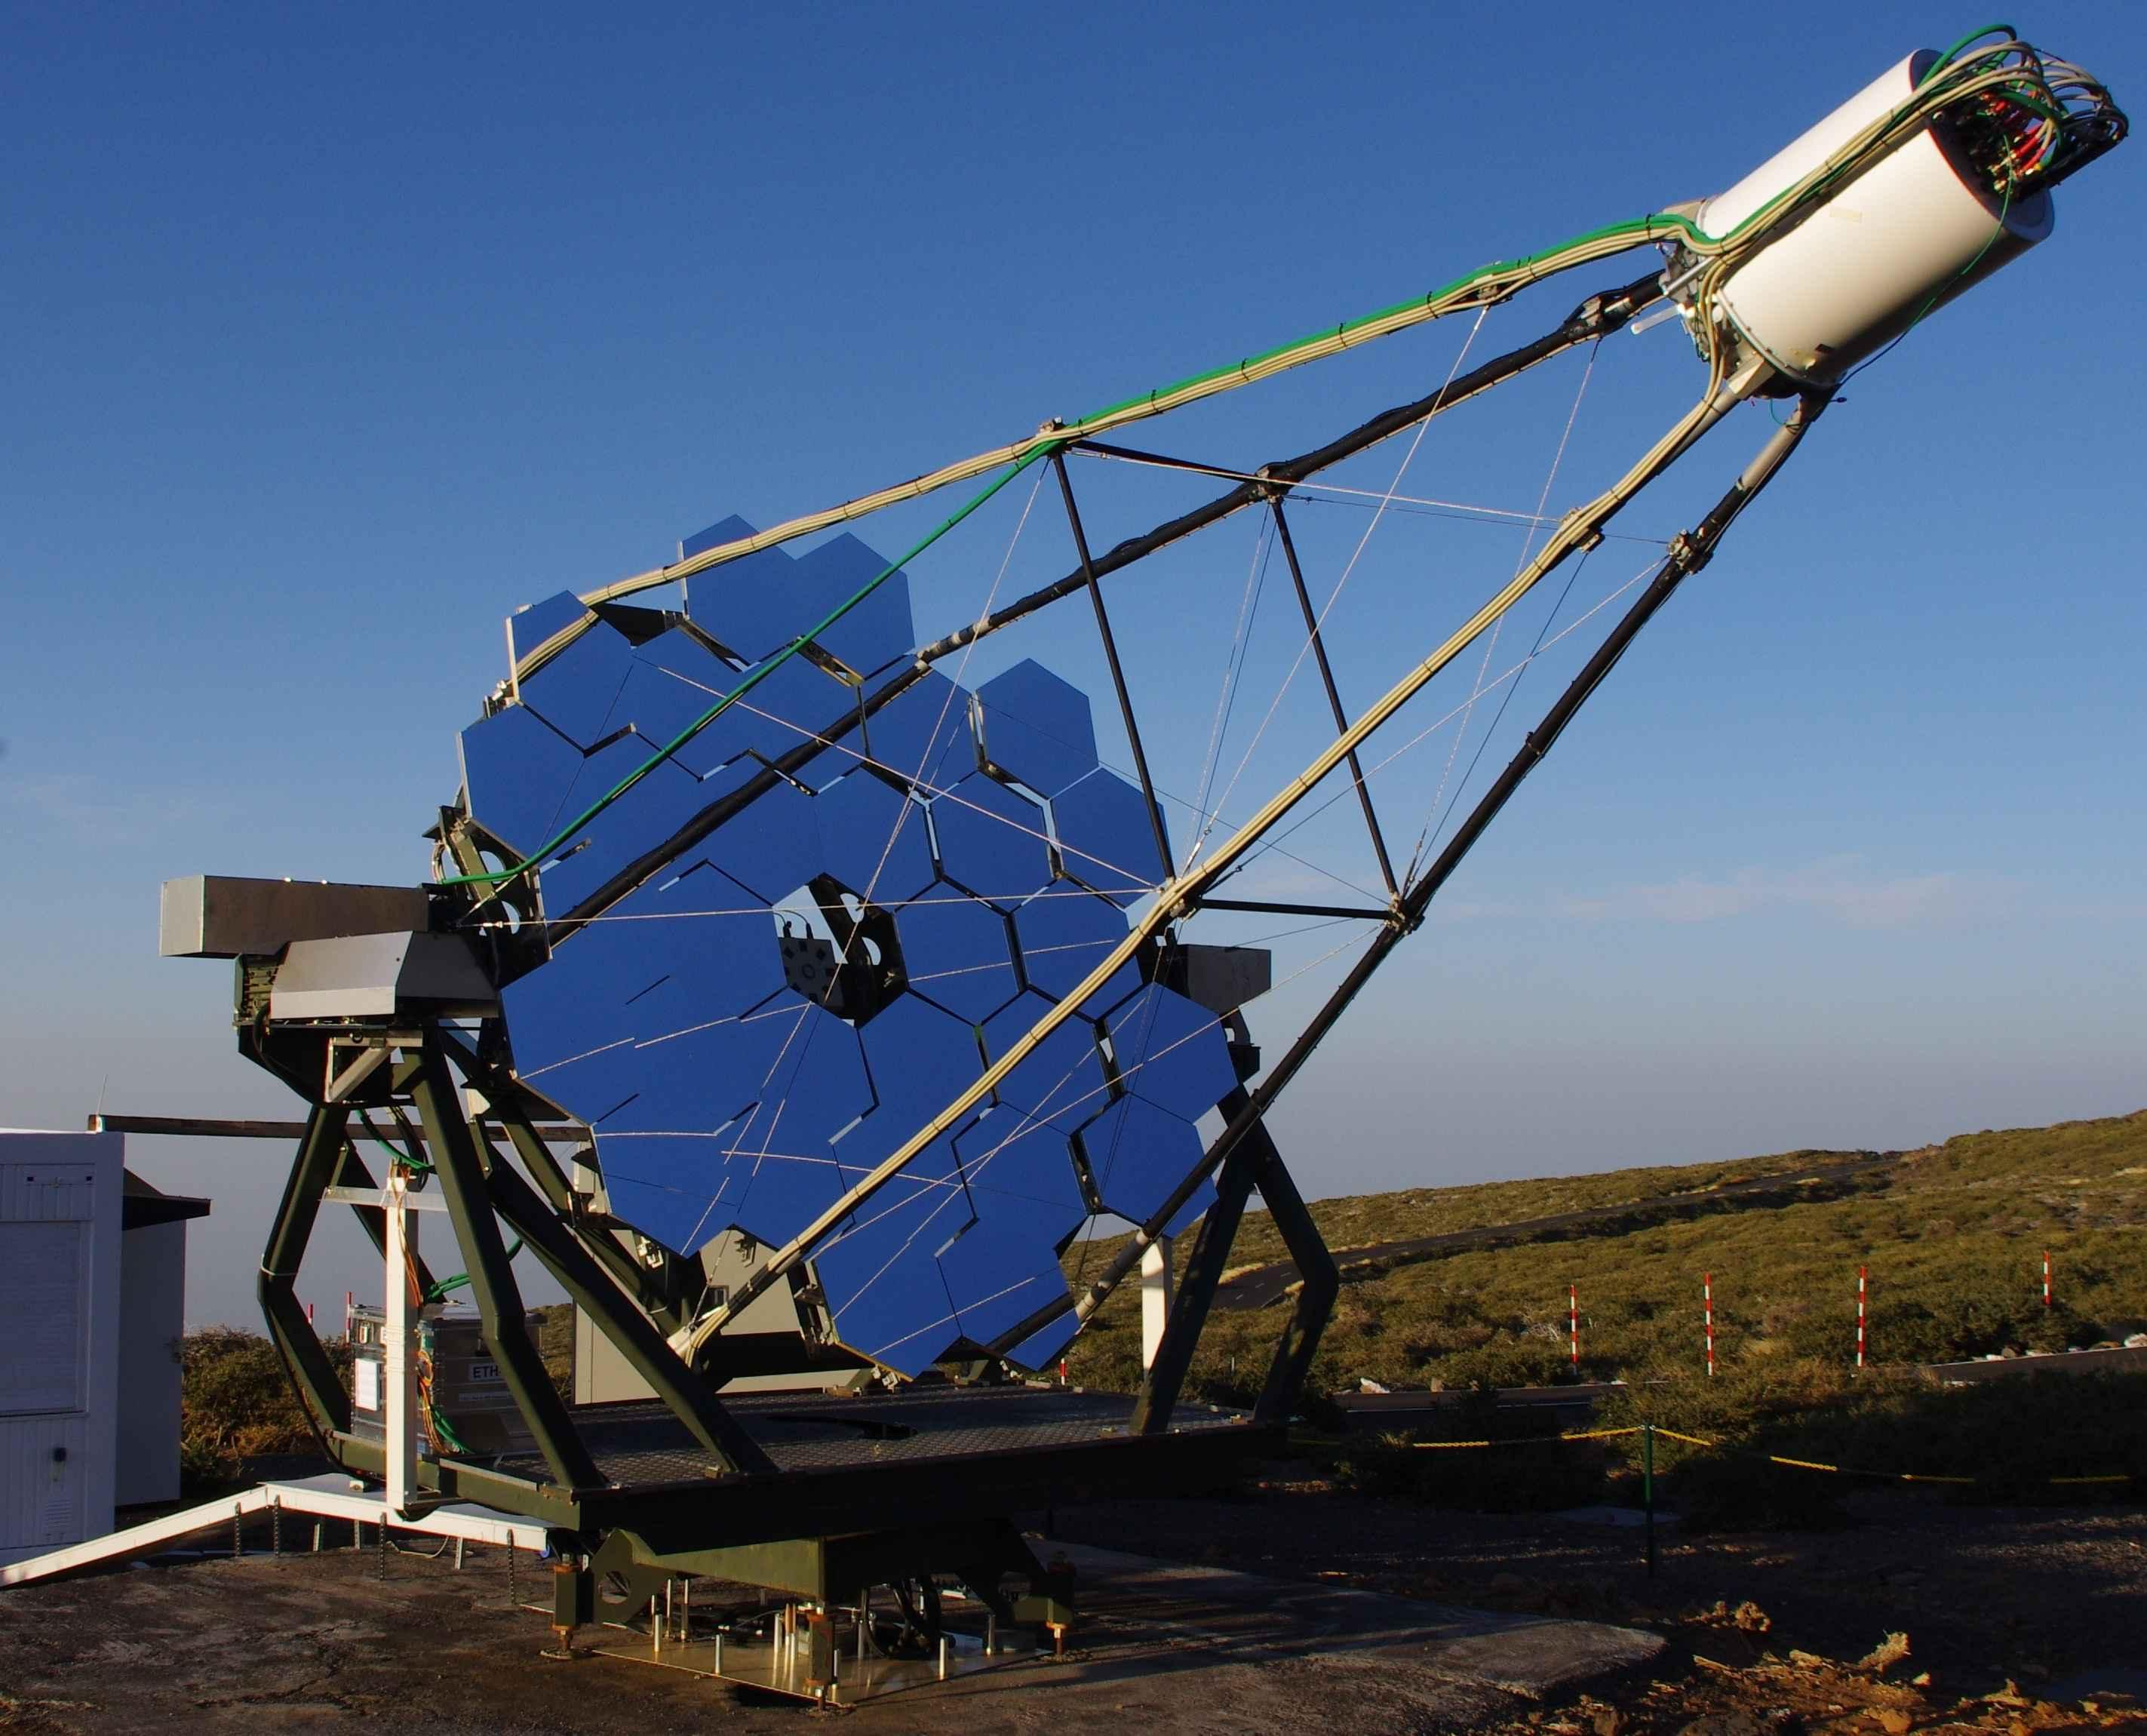
\includegraphics[width=\linewidth]{images/fact_telescope.jpg}
            \cite{Anderhub_2013}
        \end{column}
    \end{columns}
\end{frame}
